\documentclass{beamer}
\usetheme{Madrid}
\usecolortheme{seahorse}

\usepackage{graphicx}
\usepackage{booktabs}
\usepackage{amsmath}

\title{Advanced Recommender Systems for E-commerce}
\subtitle{A Comparative Study of Classical and Neural Approaches}
\author{Angsar Shaumen}
\institute{Astana IT University \\ School of Artificial Intelligence and Data Science}
\date{February 2026}

\begin{document}

% Slide 1: Title
\begin{frame}
\titlepage
\end{frame}

% Slide 2: Outline
\begin{frame}{Outline}
\tableofcontents
\end{frame}

\section{Introduction}

% Slide 3: Problem & Motivation
\begin{frame}{Problem \& Motivation}
\begin{itemize}
    \item Recommender systems are critical for e-commerce
    \item Challenge: Learning from sparse implicit feedback
    \item Question: \textbf{Do neural models outperform classical approaches?}
\end{itemize}
\vspace{0.5cm}
\textbf{Research Goal:} Compare classical (MF) vs neural (NCF) under realistic constraints
\end{frame}

% Slide 4: Research Questions
\begin{frame}{Research Questions}
\begin{enumerate}
    \item How do classical and neural recommenders compare on ranking metrics?
    \item Does NCF consistently outperform Matrix Factorization?
    \item How do models behave under extreme sparsity?
    \item What are the computational trade-offs?
\end{enumerate}
\end{frame}

\section{Dataset}

% Slide 5: Dataset
\begin{frame}{Dataset: Amazon Headphones}
\begin{columns}
\begin{column}{0.5\textwidth}
\textbf{Processing Steps:}
\begin{itemize}
    \item Filter: Headphones subcategory
    \item Implicit feedback (binary)
    \item 5-core filtering
    \item Time-based split (70/15/15)
\end{itemize}
\end{column}
\begin{column}{0.5\textwidth}
\begin{table}
\centering
\small
\begin{tabular}{ll}
\toprule
Metric & Value \\
\midrule
Users & 368 \\
Items & 282 \\
Interactions & 2,695 \\
Sparsity & 97.4\% \\
\bottomrule
\end{tabular}
\end{table}
\end{column}
\end{columns}
\end{frame}

% Slide 6: Long-tail
\begin{frame}{Data Distribution: Long-Tail Effect}
\begin{center}
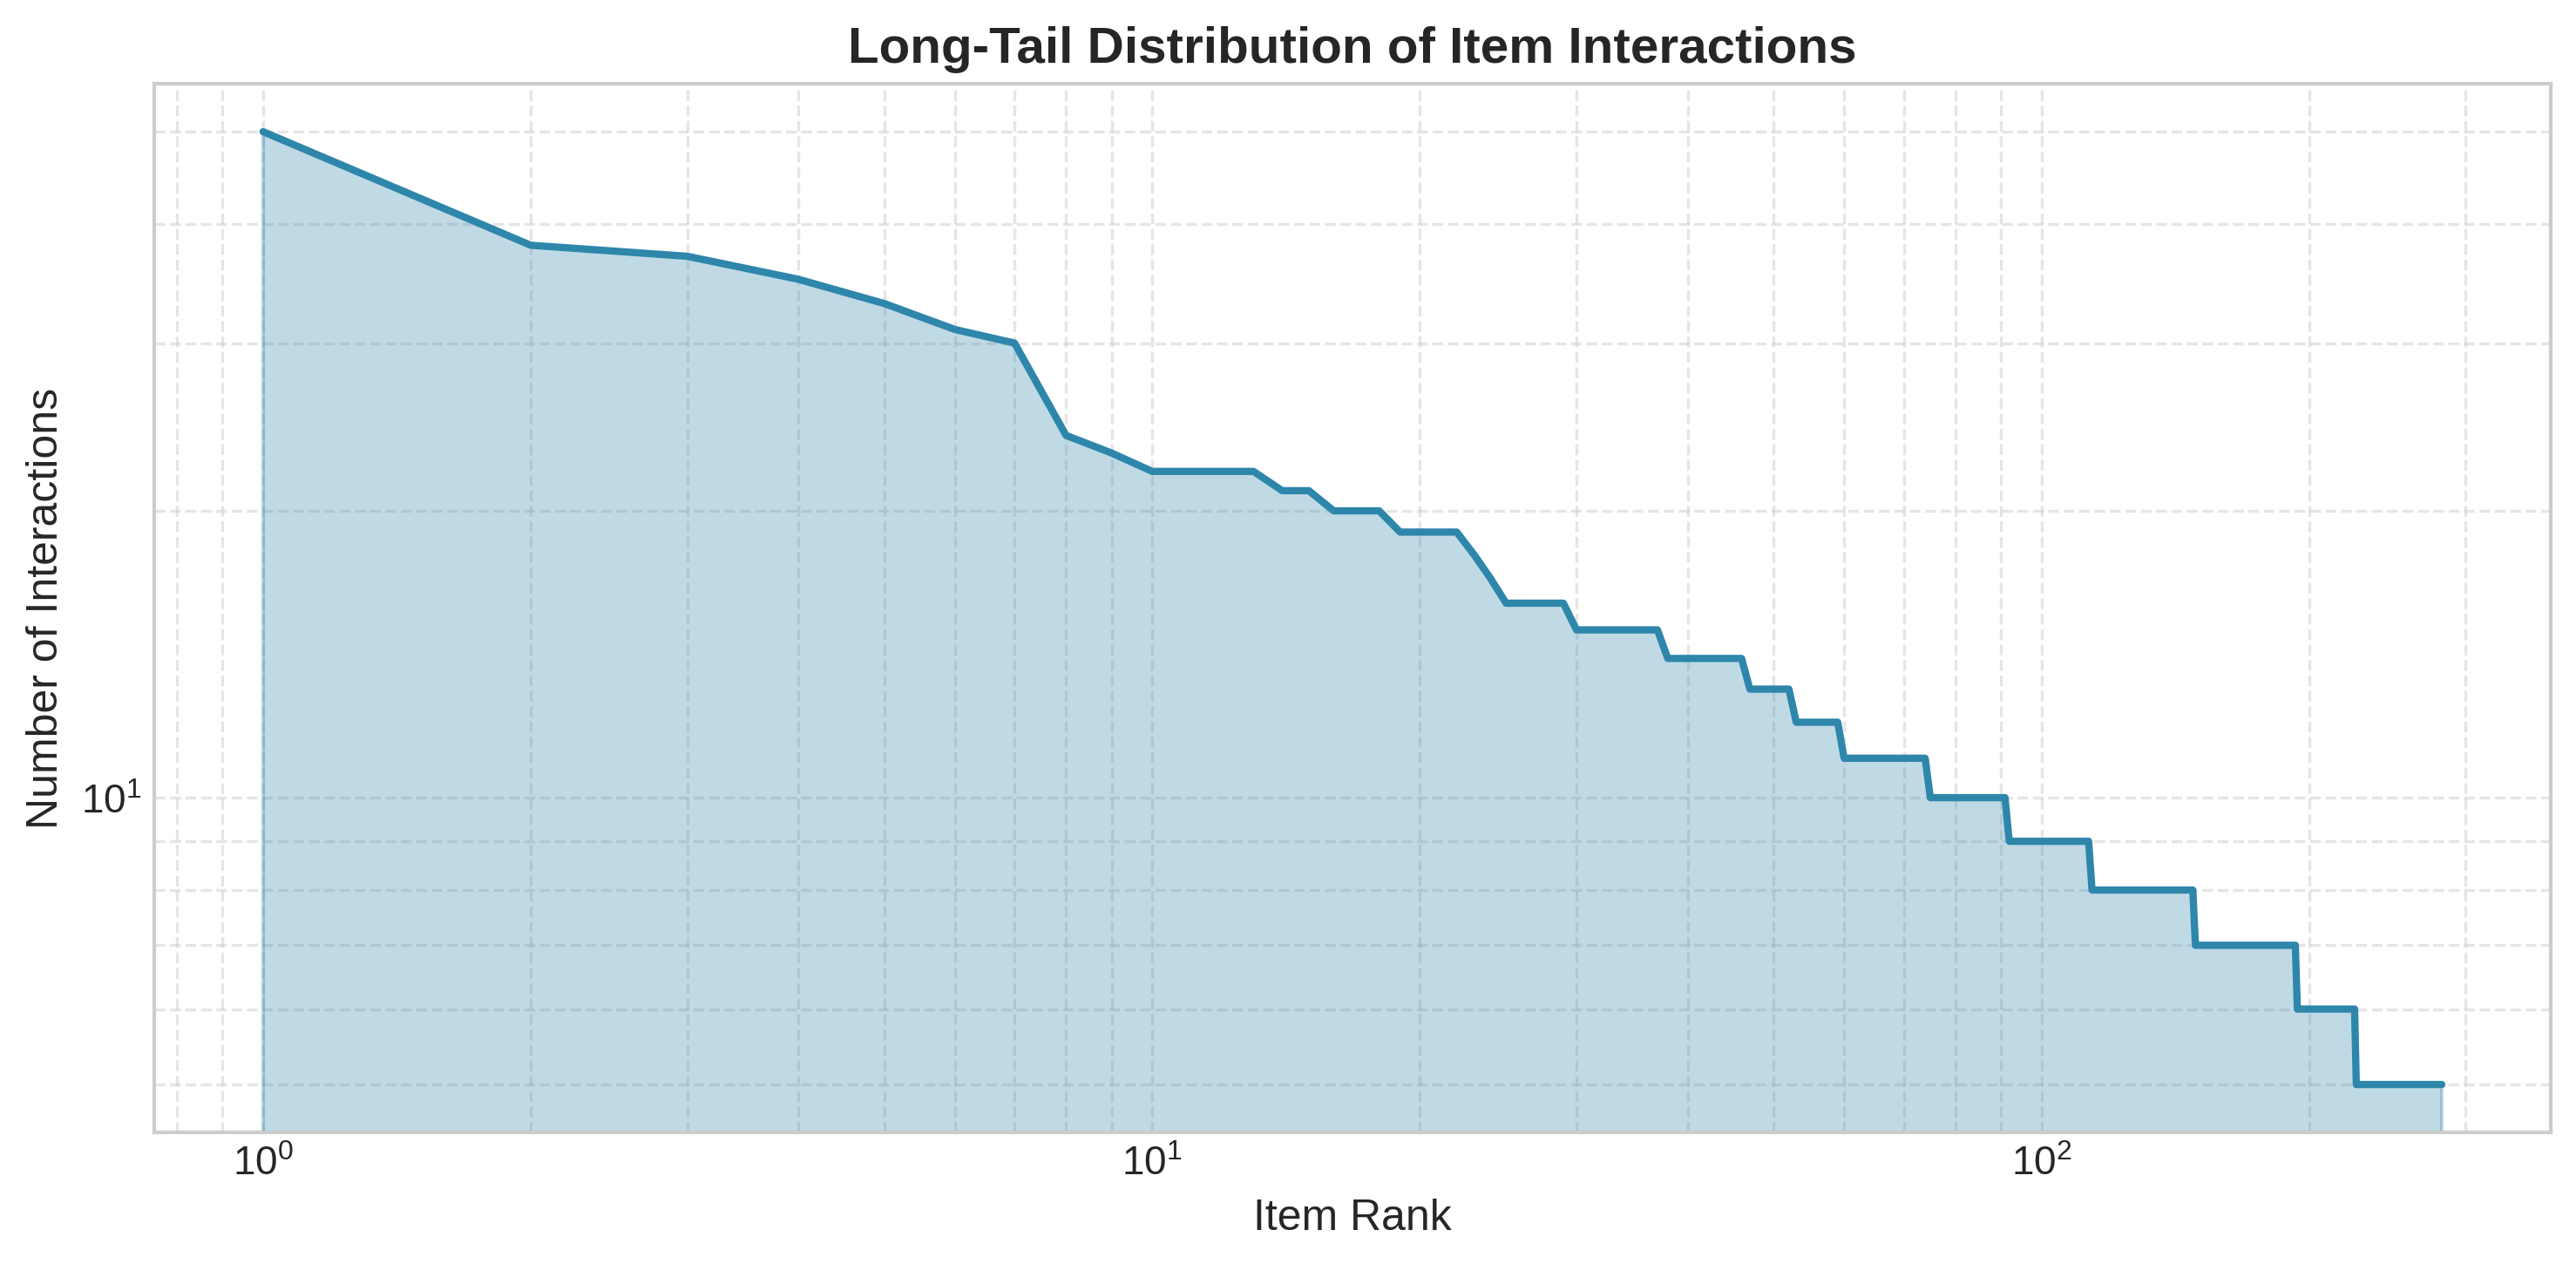
\includegraphics[width=0.8\textwidth]{figures/fig_longtail.png}
\end{center}
\textbf{Key Insight:} Few items dominate interactions
\end{frame}

\section{Methodology}

% Slide 7: Models
\begin{frame}{Models Compared}
\begin{table}
\centering
\begin{tabular}{ll}
\toprule
\textbf{Model} & \textbf{Type} \\
\midrule
Popularity & Baseline \\
Item-KNN & Collaborative Filtering \\
Matrix Factorization & Classical (Latent Factors) \\
NeuMF (NCF) & Neural Network \\
\bottomrule
\end{tabular}
\end{table}
\vspace{0.3cm}
\textbf{Evaluation:} Precision@K, Recall@K, NDCG@K
\end{frame}

% Slide 8: NCF Architecture
\begin{frame}{Neural Collaborative Filtering (NCF)}
\begin{itemize}
    \item User and Item embeddings (dim=32)
    \item GMF path: Element-wise product
    \item MLP path: Concatenation + hidden layers
    \item Final: Sigmoid output for prediction
\end{itemize}
\begin{equation*}
\hat{y}_{ui} = \sigma(h^T(\phi_{GMF} \oplus \phi_{MLP}))
\end{equation*}
\end{frame}

\section{Results}

% Slide 9: Main Results
\begin{frame}{Main Results}
\begin{table}
\centering
\small
\begin{tabular}{lcccc}
\toprule
\textbf{Model} & \textbf{P@10} & \textbf{R@10} & \textbf{NDCG@10} \\
\midrule
Popularity & 0.0023 & 0.0100 & 0.0050 \\
Item-KNN & 0.0006 & 0.0057 & 0.0020 \\
MF & 0.0017 & 0.0054 & 0.0021 \\
\textbf{NeuMF} & \textbf{0.0023} & \textbf{0.0100} & \textbf{0.0059} \\
\bottomrule
\end{tabular}
\end{table}
\vspace{0.3cm}
\textbf{Winner:} NeuMF with NDCG@10 = 0.0059
\end{frame}

% Slide 10: Visual Comparison
\begin{frame}{Model Comparison}
\begin{center}

\includegraphics[width=0.95\textwidth]{figures/fig_model_comparison.png}
\end{center}
\end{frame}

% Slide 11: Training Dynamics
\begin{frame}{Training Dynamics}
\begin{center}

\includegraphics[width=0.8\textwidth]{figures/fig_training_loss.png}
\end{center}
NCF converges slower but achieves better generalization
\end{frame}

\section{Analysis}

% Slide 12: Cold-Start
\begin{frame}{Cold-Start Analysis}
\begin{columns}
\begin{column}{0.5\textwidth}
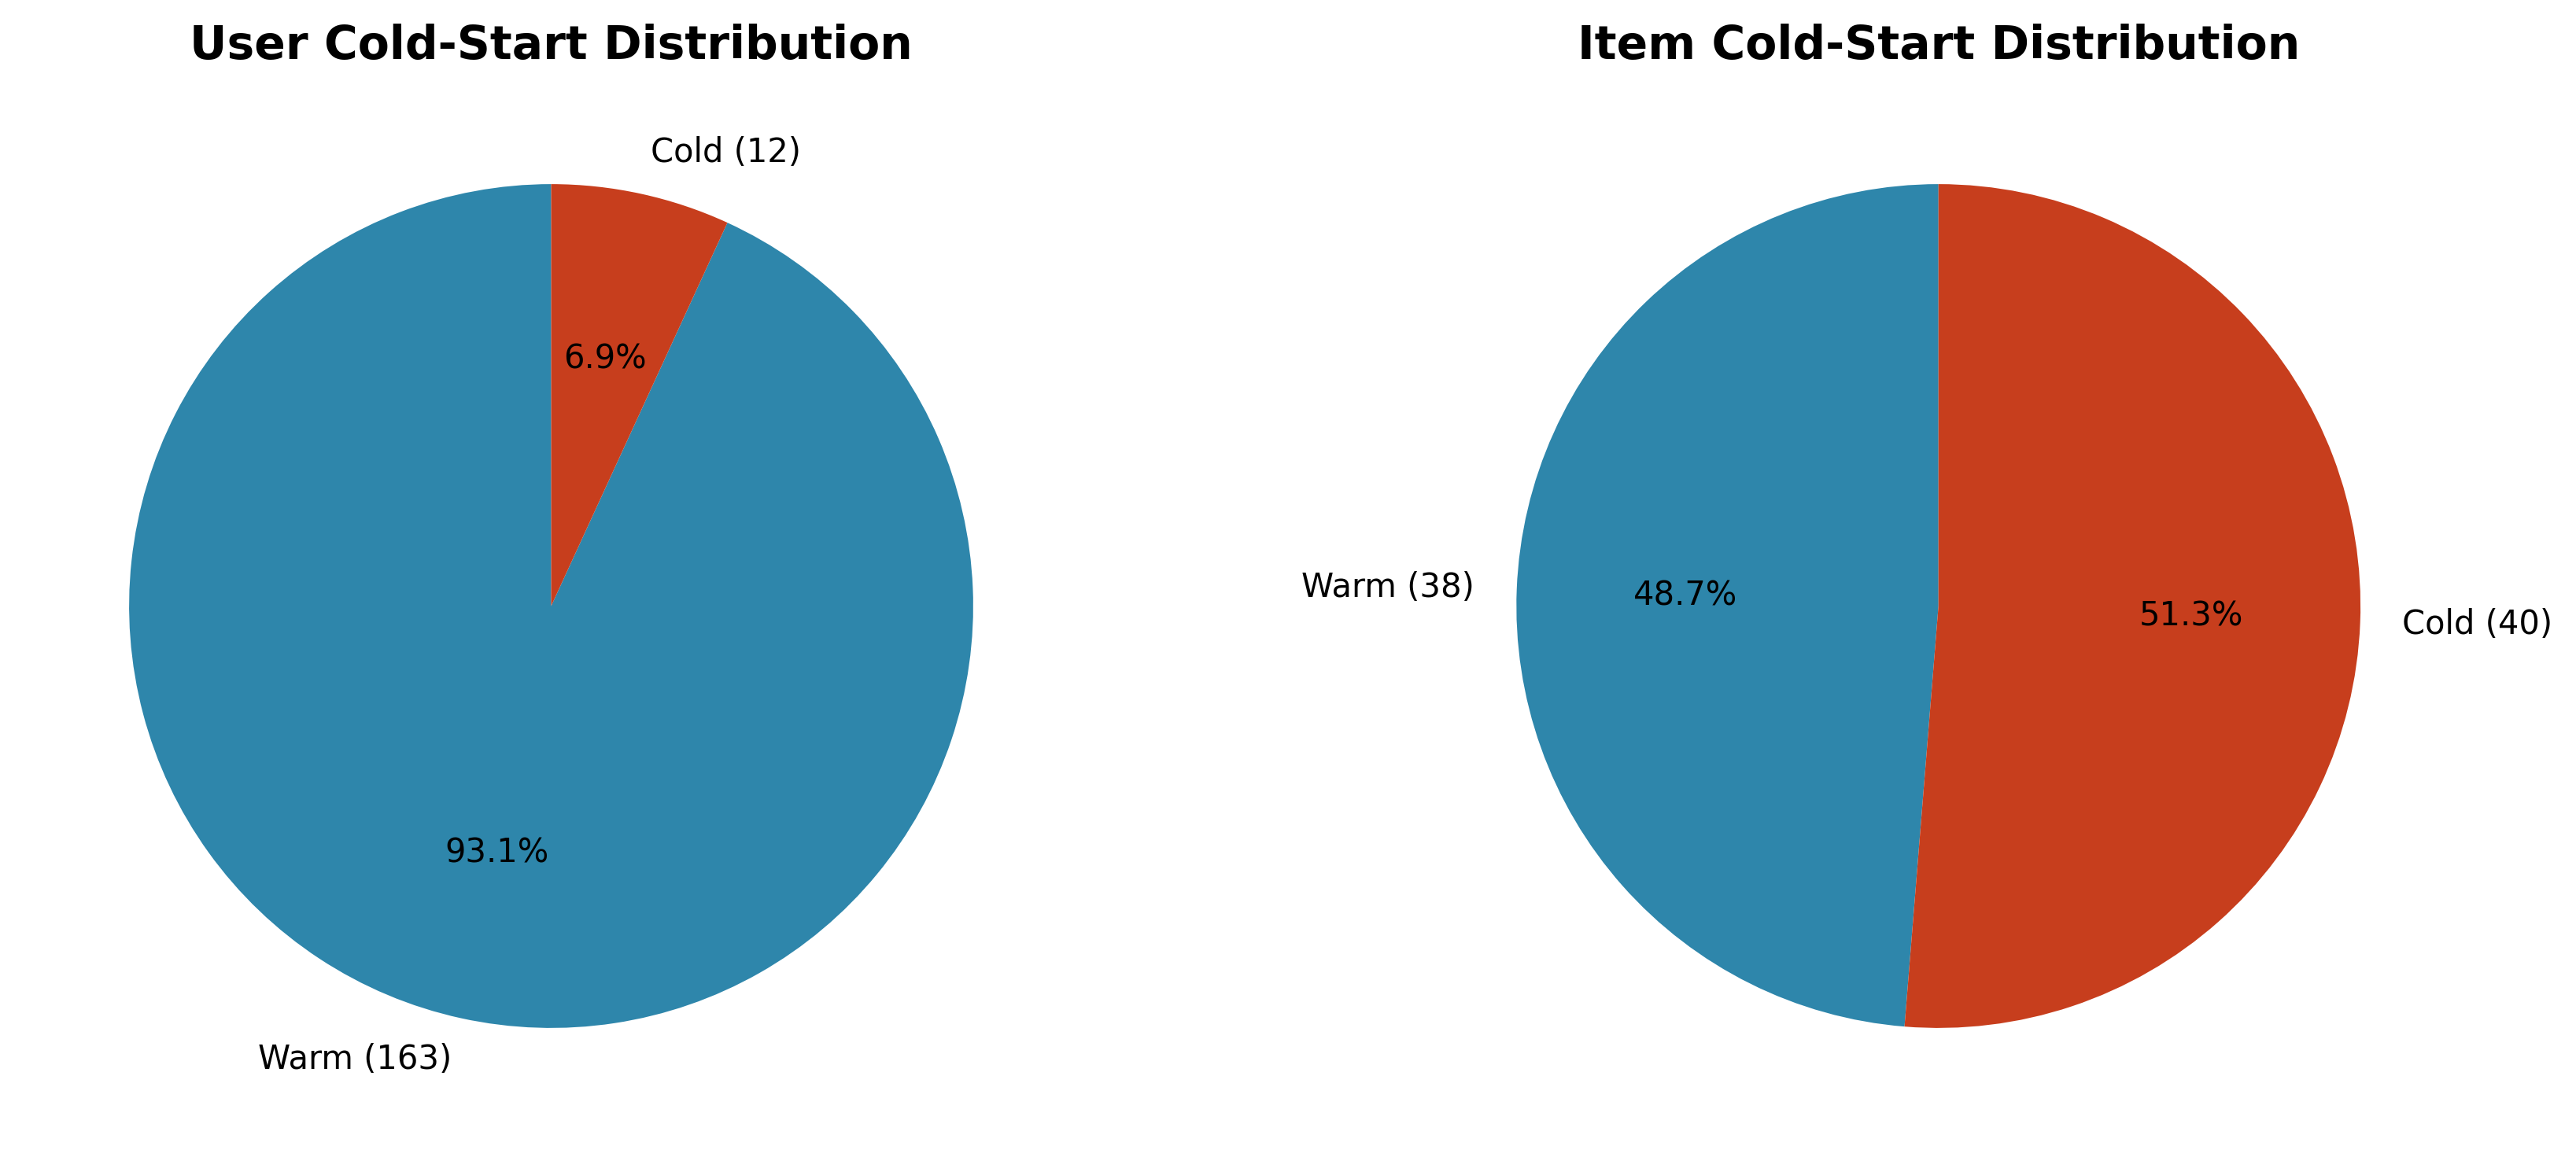
\includegraphics[width=\textwidth]{figures/fig_cold_start.png}
\end{column}
\begin{column}{0.5\textwidth}
\begin{itemize}
    \item 48.6\% cold users
    \item 51.3\% cold items
    \item Challenge for CF methods
    \item Popularity as fallback
\end{itemize}
\end{column}
\end{columns}
\end{frame}

% Slide 13: Key Findings
\begin{frame}{Key Findings}
\begin{enumerate}
    \item \textbf{NCF wins} with highest NDCG@10 (0.0059)
    \item \textbf{Sparsity hurts} classical methods more than neural
    \item \textbf{Popularity is strong} due to long-tail effect
    \item \textbf{Cold-start} affects ~50\% of test entities
\end{enumerate}
\end{frame}

\section{Conclusion}

% Slide 14: Limitations
\begin{frame}{Limitations \& Future Work}
\textbf{Limitations:}
\begin{itemize}
    \item Small dataset after filtering (2,695 interactions)
    \item No hybrid model due to limited metadata
    \item Offline evaluation only
\end{itemize}
\vspace{0.5cm}
\textbf{Future Work:}
\begin{itemize}
    \item Incorporate item features (LightFM)
    \item Sequential models (SASRec, BERT4Rec)
    \item Online A/B testing
\end{itemize}
\end{frame}

% Slide 15: Conclusion
\begin{frame}{Conclusion}
\begin{block}{Summary}
Neural Collaborative Filtering (NCF) outperforms classical Matrix Factorization in highly sparse e-commerce data, demonstrating the value of non-linear interaction modeling.
\end{block}
\vspace{0.5cm}
\textbf{Code \& Data:} Available in the accompanying repository
\end{frame}

% Slide 16: References
\begin{frame}{References}
\footnotesize
\begin{itemize}
    \item He et al. (2017). Neural Collaborative Filtering. WWW.
    \item Koren et al. (2009). Matrix Factorization Techniques. IEEE Computer.
    \item Rendle et al. (2009). BPR: Bayesian Personalized Ranking. UAI.
    \item Hu et al. (2008). Collaborative Filtering for Implicit Feedback. ICDM.
    \item Sarwar et al. (2001). Item-based Collaborative Filtering. WWW.
\end{itemize}
\end{frame}

% Slide 17: Thank You
\begin{frame}
\begin{center}
\Huge Thank You!\\
\vspace{1cm}
\Large Questions?
\end{center}
\end{frame}

\end{document}
